\documentclass[11pt]{scrartcl}
\usepackage[utf8]{inputenc} % Kodierung der Textdatei mit Sonderzeichen
\usepackage[ngerman]{babel} % Sprache fuer Inhaltsverzeichnis etc.
\usepackage{amssymb} % Mathematische Symbole
\usepackage{amsmath} % Mehr mathematische Konstrukte
\usepackage{graphicx} % Um Bilder einbinden zu koennen
\usepackage{float} % fuer \begin{figure}[H]
\usepackage{icomma} % laesst das Komma als Dezimaltrennzeichen interpretieren



\newcommand{\unit}[1]{\ensuremath{\,\mathrm{#1}}} % Einheiten schreiben sich immer aufrecht!
\newcommand{\degr}{\ensuremath{^\circ}}
\newcommand{\cel}{\ensuremath{\degr\mathrm{C}}}
\newcommand{\dif}{\ensuremath{\mathrm{d}}}
\newcommand{\pdif}[2]{\ensuremath{\frac{\partial#1}{\partial#2}}}
\newcommand{\ee}[1]{\ensuremath{\cdot 10^{#1}}}


\setlength{\parindent}{0pt}
\setlength{\parskip}{0.5\baselineskip}


\title{Gr\"atzelzelle - Gruppe 5 WS 09/10, Projektpraktikum der Uni Erlangen}
\date{19.10.2009 -- 31.10.2009}
\author{Michele Collodo, Andreas Glossner, Karl-Christoph G\"odel, Bastian Hacker, Maria Obst, Alexander Wagner, David Winnekens}



\begin{document}
\sloppy % laesst Latex nicht ueber den Rand rausschreiben
\thispagestyle{empty}
\large{Projektpraktikum WS 09/10}
\hfill
\raisebox{-1.4cm}{
\includegraphics[width=5cm]{images/fau.pdf}}
\\[8\baselineskip]
\begin{center}
{\Huge\textbf{Gr\"atzelzelle}}
\\[0.5\baselineskip]
{\large Energieforschung auf der Nanoebene}
\\[1.5\baselineskip]
{\Large 19.10.2009 -- 31.10.2009}
\\[6\baselineskip]
{\Huge\textbf{PPG 5}}\\[0.5\baselineskip]
{\large\textbf{
Michele Collodo,
Andreas Glossner,\\
Karl-Christoph G\"odel,
Bastian Hacker,\\
Maria Obst,
Alexander Wagner,
David Winnekens}\\
Tutor: Xiaoyue Jin}
\vfill



\small{\texttt{http://pp.physik.uni-erlangen.de/groups/ws0910/ppg5/ppg5\_start.html}}
\end{center}
\newpage



\tableofcontents
\vfill



\begin{abstract}
%%% Maria

Pr\"agnante Beschreibung was wir gemacht haben \ldots
\end{abstract}
\newpage





\section{Einleitung}
relativ kurz \ldots





\section{Theorie}
\subsection{B\"andermodell und Halbleitertechnik}
Um die Funktionsweise von Solarzellen im allgemeinen und der Gr\"atzelzelle im besonderen verstehen zu k\"onnen, muss man sich zun\"achst mit dem Energieb\"andermodell aus der Quantenmechanik besch\"aftigen. Die B\"ander entstehen durch \"Uberlagerung der Energieniveaus der einzelnen, im Kristall dicht nebeneinander gelagerten Atome. Nahe bei den Atomr\"umpfen befinden sich die gebundenen Zust\"ande. Wenig dar\"uber entsteht durch \"Uberlappung der Potentiale das Valenzband, in dem alle Pl\"atze mit Elektronen besetzt sind. So kann sich ein Elektron nur bewegen, wenn sich ein anderes Elektron genau in entgegengesetzter Richtung bewegt. 
Noch weiter von den Atomr\"umpfen entfernt liegen weitere, unbesetzte Energieniveaeus \"ubereinander. Hier k\"onnen sich die Elektronen frei bewegen, dieses Band wird daher Leitungsband genannt

Zwischen Valenz- und Leitungsband befindet sich die verbotene Zone (Bandl\"ucke), in der sich keine Elektronen befinden. Nach der Gr\"o\ss{}e dieser Zone unterscheidet man Leiter, Halbleiter und Isolatoren. Bei einem Leiter gibt es keine verbotene Zone und Valenz- und Leitungsband gehen ineinander \"uber oder im Valenzband sind nicht alle Pl\"atze mit Elektronen besetzt. So kann problemlos Strom fliessen. Isolatoren hingegen haben ein vollst\"andig besetztes Valenzband und die Bandl\"ucke ist so gro\ss{} dass sie selbst von hoch angeregten Elektronen nicht oder nur sehr schwer \"uberwunden werden kann.

Auch bei Halbleitern ist das Valenzband voll besetzt, jedoch ist hier die verbotene Zone noch kleiner als etwa 10eV. Es ist also f\"ur Elektronen, die durch hohe Temperaturen oder einfallende Photonen angeregt sind, m\"oglich, die L\"ucke zu \"uberspringen und sich im Leitungsband fortzubewegen. Werden hier nun in den Kristall Fremdatome eingef\"ugt (Dotierung), ver\"andern sich dessen leitenden Eigenschaften. Werden Atome eingesetzt, die mehr Elektronen in der \"au\ss{}eren Schale haben als die des Kristalls (n-Dotierung), so gibt es \glqq\"ubersch\"ussige\grqq Elektronen, die einfacher ins Leitungsband wechseln k\"onnen. Solche Atome hei\ss{}en Elektronendonatoren. F\"ugt man hingegen Fremdatome ein, die weniger Elektronen in ihrer \"au\ss{}eren Schale haben (p-Dotierung), entstehen L\"ocher, in denen leicht Elektronen aus dem Valenzband angelagert werden. Es gibt nun Elektronenfehlstellen, die Atome werden als Elektronenakzeptoren bezeichnet.

Bringt man nun einen p-dotierten und einen n-dotierten Halbleiter zusammen, diffundieren die \"ubersch\"ussigen Elektronen aus der n-Schicht zu den Fehlstellen in der p-Schicht, es bildet sich ein elektrisches Feld, das von der n- zur p-Seite gerichtet ist. Nun k\"onnen durch das Anlegen einer \"au\ss{}eren Spannung verschiedene Funktionen, wie beispielsweise die Diode, erreicht werden. Schliesst man den Pluspol an die p-Schicht und den Minuspol an die n-Schicht, betreibt man eine Diode in Durchlassrichtung. Die Bandl\"ucke wird beinahe aufgehoben und Leitung ist m\"oglich.

Bei umgekehrter Polung, also in Sperrichtung, kann kein Strom flie\ss{}en. Solche Dioden nennt man Photodioden, sie werden in herk\"ommlichen Solarzellen verwendet. Eine Gr\"atzelzelle hingegen greift mehr auf Ideen der Natur zur\"uck. Hier wird durch Imitation der nat\"urlichen Photosynthese Energie erzeugt.



\subsection{Funktionsweise der Gr\"atzelzelle}
Die Gr\"atzelzelle, benannt nach ihrem Erfinder, dem Schweizer Michael Gr\"atzel, besteht aus zwei Elektroden, typischerweise leitend beschichtete Glasplatten. Auf der einen Glasplatte wird als Halbleiter Titandioxid angebracht. Da hier aber die verbotene Zone aber eine Gr\"o\ss{}e von 3.2eV hat, w\"are die Zelle nur f\"ur hochenergetische Photonen des UV-Lichts empfindlich. Daher wird auf die TiO$_{2}$-Schicht ein lichtempfindlicher organischer Farbstoff aufgebracht, dessen Elektronen auch von sichtbarem Licht angeregt werden k\"onnen. Die Gr\"atzelzelle wird deshalb auch als Farbstoffsolarzelle bezeichnet.

Die Gegenelektrode ist mit einem Katalysator, oft Platin, beschichtet, um die \"Ubergabe der ausgel\"osten Elektronen zu erleichtern. Den Raum zwischen den beiden Elektroden f\"ullt ein Elektrolyt, der in Redox-Reaktionen einerseits dem Farbstoff schnellen Nachschub an Elektronen liefert und andererseits an der Kathode wieder zur\"uck reagiert. Hier wird h\"aufig Iodkaliumiodid eingesetzt.





\section{Aufbau}
\subsection{Materialien, Beschaffung und Bau der Zelle}
%%% Karl
Die Beschaffung der f\"ur den Bau ben\"otigten Materialien stellte zu Beginn ein Problem dar. Insbesondere war es schwer, leitende und gleichzeitig transparente Elektroden zu bekommen. Die erste M\"oglichkeit, mit Gold beschichtet Glaspl\"attchen, zu verwenden, scheiterte an den zu geringen Ausma\ss{}en der m\"oglichen Tr\"agerplatten. Zu lange Lieferzeiten und zu hohe Preise schlossen auch die Bestellung von industriell produzierten ITO-Gl\"asern (Indiumzinnoxid-Beschichtung) aus.

Das Institut der Physikalischen Chemie der Universit\"at Erlangen stellte gl\"ucklicherweise mehrere Fluorzinnoxid (FTO) beschichtete Glasplatten zur Verf\"ugung. Die leitend beschichteten, transparenten Glasplatten waren bereits auf eine Gr\"o\ss{}e von \(70\unit{mm} \times 20\unit{mm} \times 4 \unit{mm}\) zugeschnitten. Auf der leitenden Seite der Glasplatte konnte mit Hilfe eines Multimeters ein Widerstand von etwa \(20 \unit{\frac{\Omega}{cm}}\) gemessen werden.

Das Elektrolyt, eine Iod-Kaliumiodid-L\"osung sowie verd\"unnte Salzs\"aure zum Anmischen der Titandioxidpaste konnten ebenfalls von der Physikalischen Chemie bezogen werden.



\subsection{Versuchsanordnung} %%% Michele und Axi
%%% noch weiter untergliedern? vorueberlegung, LED, Wellenlaenge, Leistung? -> eher nein
Das erste Ziel war die Bestimmung der Abh\"angigkeit der Leistung der Zelle von der Wellenl\"ange des eingestrahlten Lichts. Zun\"achst wollten wir dieses Spektrum mit einem Gitter erzeugen. Die ersten Versuche mit einem Aufbau aus Baustrahler, Linse und Gitter auf einer optischen Bank hatten jedoch bereits gezeigt, dass die zu erwartende Lichtst\"arke des aufgef\"acherten Spektrums viel zu schwach f\"ur eine Messung sein w\"urde. Au\"sserdem wurden die einzelnen Linien des Spektrums viel zu schwach aufgef\"achert, so dass nicht nur ein Farbbereich auf die breitere Zelle treffen w\"urde. Auch der Ersatz des Gitters durch ein Prisma konnte diese Probleme nicht l\"osen.

Deshalb haben wir uns entschlossen, die verschiedenen Farbbereiche durch LEDs unterschiedlicher Wellenl\"ange darzustellen. Hierbei kam ein Verbund aus zehn verschiedenen LEDs zum Einsatz, welcher bereits fr\"uher von einem Gruppenmitglied gebaut wurde.
%%% Beschreibung der LEDs, Wellenlaengen? , Spannungen? 
Die LEDs sind einzeln dimmbar, sie wurden jedoch stets bei maximaler Leuchtst\"arke betrieben.

Um eine Vergleichmessung wie die Wellenl\"angenabh\"angigkeit genau durchf\"uhren zu k\"onnen, muss der Aufbau bei jeder Einzelmessung genau gleich sein. Daf\"ur wurde die Gr\"atzelzelle in eine Halterung aus Klemmen und Stativstangen eingespannt. Der Verbund aus LEDs wurde entlang der Grundplatte des Aufbaus unter die Zelle geschoben. Zwischen LED und Zelle kam eine variable Blende zum Einsatz, deren \"Offnungsdurchmesser fest auf ca. $1,8\unit{cm}$ eingestellt war. Eine weitere Stativstange markierte dabei die Stelle, an der sich die momentan verwendete LED befinden musste, um jeweils genau senkrecht unter Zelle positiniert zu sein. Der vertikale Abstand LED - Zelle betrug dabei ca. $12\unit{cm}$.

In der selben H\"ohe wurde, versetzt zur Zelle, auch ein LUX-Seonsor befestigt, um eine Messung der jeweiligen Leuchtkraft der LEDs zu erm\"oglichen. Auch hier markierte eine Stativstange die Messposition. Zum Auslesen des Sensor wurde das CASSY-LAB verwendet, welches die Messwerte \"uber $1000\unit{ms}$ gemittelt anzeigte.

Die Messung, der von der Zelle gelieferten Spannung, erfolgte zum Einen durch ein direkt an die Zelle angeschlossenes Multimeter, sowie durch ein weiteres Multimeter, dessen Signal jedoch zun\"achst einen Messverst\"arker durchlief. Der genau Aufbau ist auch aus dem folgenden Schaltplan sowie dem Foto ersichtlich.\newline
hier fehlt Schaltplan + Foto

Bei der Messung wurde jeweils zwei Minuten gewartet, bis sich die Messwerte eingependelt hatten.
%%% gehoert das hier hin?

Der zweite Teil der Messung umfasste die Bestimmung der Leistung der Solarzelle in verschiedenen Widerstandsbereichen. Hierbei wurde nur die LED Nr.7 (Farbe blau) verwendet, da sie die h\"ochsten Spanungen geliefert hat. Au\ss{}erdem kam eine neue Gr\"atzelzelle zum Einsatz, da die Zelle der ersten Messung bereits eingetrocknet war.

Der Aufbau der LEDs wurde leicht angepasst. Neben einem geringeren Abstand der Lichtquelle von der Zelle, ersetzte eine Linse die Lochblende zum Fokussieren des Lichtsstrahls.

Die Messung der Strom- und Spannungswerte wurde mit einem Multimeter f\"ur die Spannung und einem Amperemeter f\"ur die Stromst\"arke durchgef\"uhrt. Der Einsatz eines Messverst\"arkers war hierbei nicht m\"oglich, da die anschlie\ss{}end am Multimeter abzulesenden Werte sehr starke Schwankungen aufwie\ss{}en und einen Offset unklaren Ursprungs enthielten.

Der Aufbau sowie die verwendeten Bauteile sind wiederum im Schaltplan (Abb.~\ref{leistungsschaltkreis}) sowie den Foto illustriert:

\begin{figure}[ht]
\begin{center}
%%% Zeichnung mit xcircuit
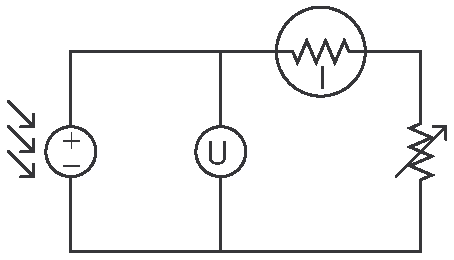
\includegraphics[width=0.8\textwidth]{images/leistungsmesskreis.pdf}
\end{center}
\vspace{-1.5\baselineskip}
\caption{Schaltkreis zur Leistungsmessung. Das Amperemeter hatte einen signifikaneten Eigenwiderstand.}
\label{leistungsschaltkreis}
\end{figure}
hier fehlt Foto

Um mehrere Paare an Messwerten zu erhalten, wurde wie zu sehen ist, ein regelbarer Widerstand zwischengeschalten und die Messung mit verschiedenen Kombinationen der Widerst\"ande durchgef\"uhrt. Leider hatte auch das Amperemeter einen Eigenwiderstand. Dieser hat allerdings die Messmethode nicht nachhaltig beeinflusst. ($\rightarrow$ vgl. Ergebnisse) %%% gehoert das hier hin?





\section{Messungen und Ergebnisse}
%%% Basti, Michele (LED's)
\subsection{Leistung und Wirkungsgrad}
Zur Leistungsmessung wurden die Strom- und Spannungswerte der Zelle mit einer spannungsrichtigen Schaltung nach (Abb.~\ref{leistungsschaltkreis}) bei verschiedenen Lastwiderständen gemessen. Die Lastwiderstände waren über eine Kombinationsbox einstell- und ablesbar. Das Voltmeter hatte mit $10\unit{M\Omega}$ genügend Eigenwiderstand um die Messung nicht zu beeinflussen. Das Amperemeter hatte jedoch wegen der hohen benötigten Empfindlichkeit einen signifikanten Eigenwiderstand von
\[
R_I = 5,22\pm 0,03 \unit{k\Omega}
\qquad\qquad\qquad
R = R_I+R_{\text{L}}\;.
\]
Der zusätzliche Lastwiderstand $R$ wurde nun im Bereich 0 -- $40\unit{k\Omega}$ variiert und jeweils wenige Minuten gewartet bis sich stationäre Werte einstellten. Die Messwerte stehen in Tabelle \ref{leistungsmesstabelle}.
\begin{table}[ht]
\captionabove{Messwerte zur Leistungsbestimmung}
\begin{center}
\begin{tabular}{rr|ccc}
$R_{\text{L}}[\unit{k\Omega}]$ &
$R [\unit{k\Omega}]$ &
$U [\unit{mV}]$ &
$I [\unit{\mu A}]$ &
$P [\unit{nW}]$ \\
\hline
0	& 5,2	& 34,5	& 6,2	& 214 \\
1	& 6,2	& 38,0	& 5,9	& 224 \\
5	& 11,2	& 52,4	& 5,1	& 267 \\
10	& 16,2	& 66,0	& 4,3	& 284 \\
15	& 21,2	& 75,1	& 3,7	& 278 \\
20	& 26,2	& 82,3	& 3,2	& 263 \\
25	& 31,2	& 88,8	& 2,9	& 258 \\
30	& 36,2	& 93,3	& 2,6	& 243 \\
35	& 41,2	& 96,5	& 2,4	& 232 \\
40	& 46,2	& 99,7	& 2,3	& 229
\end{tabular}
\end{center}
\label{leistungsmesstabelle}
\end{table}
Die Ableseungenauigkeit durch die begrenzte Anzeigegenauigkeit und Messwertschankungen betrugen:
\[
\Delta R_I = 0,03\unit{M\Omega}
\qquad\quad
\Delta R_{\text{L}} = 1\% R
\qquad\quad
\Delta U = 1\unit{mV}
\qquad\quad
\Delta I = 0,2\unit{\mu A}
\]
Die größte Ungenauigkeit lag also im Messen der winzigen Ströme.

Der Leistungsverlauf zeigt ein Maximum bei mittleren Widerständen (im Bereich des Eigenwiderstandes der Zelle). Bei geringen Widerständen wird die meißte Leistung in der Zelle selbst freigesetzt und bei hohen Widerstand sorgt der geringe Stromfluss für eine schlechte Leistungsausbeute.
\begin{figure}[ht]
\begin{center}
%%% Zeichnung mit xcircuit
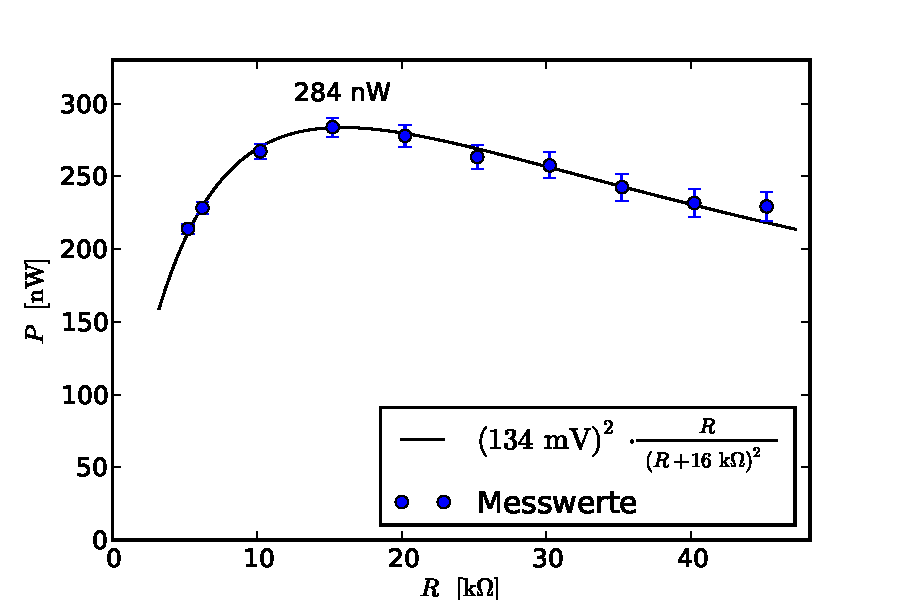
\includegraphics[width=1.0\textwidth]{images/graetzel_leistung.pdf}
\end{center}
\vspace{-1.5\baselineskip}
\caption{Leisungskurve in Abhängigkeit vom äußeren Widerstand. Auf die Daten wurde das Modell einer widerstandsbehafteten Spannungsquelle gefittet.}
\label{leistungskurve}
\end{figure}
Abb. \ref{leistungskurve} zeigt den Verlauf der Spannung zusammen mit dem Modell einer widerstandsbehafteten Spannungsquelle. Der theoretische Leistungsverlauf wäre hier:
\[
P(R)= U_{\text{Last}}\cdot I
= U_{\text{Last}}\cdot \frac{U_{\text{Zelle}}}{R+R_{\text{Zelle}}}
\]
\[
= \left(U_{\text{Zelle}}\cdot \frac{R}{R+R_{\text{Zelle}}}\right)\cdot \frac{U_{\text{Zelle}}}{R+R_{\text{Zelle}}}
= U_{\text{Zelle}}^2\cdot \frac{R}{(R+R_{\text{Zelle}})^2}
\]
Auf die Messdaten wurden nun die Zellspannung $U$ und der Eigenwiderstand $R_{\text{Zelle}}$ gefittet. Die Best-fit Werte sind:
\[
U = 134\unit{mV}
\qquad\qquad
R_{\text{Zelle}} = 15,9\unit{k\Omega}
\]
Die Spannung erreicht hier einen sehr zufriedenstellenden Wert im $0,1\unit{V}$ Bereich, also in der Größenordnung kommerzieller Zellen. Der Innenwiderstand von ca. $16\unit{k\Omega}$ ist jedoch viel zu groß um eine vernünftige Leistung zu erzeugen. Hierdurch konnte die Zelle im Endeffekt auch nicht wirklich "`unter Last"' getestet werden und die tatsächliche Leistungsfähigkeit von Grätzelzellen entzieht sich unserer Untersuchung.

Die Eingestrahlte Leistung in diesem Versuchsteil ermittelt sich aus den verwendeten Leuchtdioden \ldots
% Michele hier die eingestrahlte Leistung ausrechnen.

Unser tatsächlich erreichter Wirkungsgrad liegt also bei \ldots

\subsection{Wellenl\"ange}





\section{Fazit}
%%% zusammen
Dank an Vito Wieauchimmer, etc.
\end{document}

